\documentclass[aspectratio=169]{beamer}

\usetheme{Madrid}
\usecolortheme{whale}

\usepackage[utf8]{inputenc}
\usepackage{graphicx}
\usepackage{amsmath}
\usepackage{amssymb}
\usepackage{booktabs}
\usepackage{hyperref}

\setbeamertemplate{navigation symbols}{}

\title{InfoGeometry Lean 4}
\subtitle{Architecture, Verified Bridges, and LLM/PDE Extensions}
\author{InfoGeometry Library Team}
\date{\today}

\begin{document}

\begin{frame}
  \titlepage
\end{frame}

\begin{frame}{Presentation Goals}
  \tableofcontents
\end{frame}

\section{Audit and Scope}

\begin{frame}{What Was Missing in the Previous Deck}
  \begin{itemize}
    \item \textbf{Narrow scope}: only KL/Fisher/entropy snapshots, no architecture map.
    \item \textbf{Weak depth}: did not show verified bridge theorems across modules.
    \item \textbf{No systems view}: omitted canonical/research layering and promotion path.
    \item \textbf{No AI stack view}: did not surface the new LLM formal interfaces.
    \item \textbf{No geometric flow layer}: Ricci/Monge-Ampere additions were absent.
  \end{itemize}
  \vspace{0.5em}
  This revision addresses each gap with module-level coverage and bridge-focused figures.
\end{frame}

\begin{frame}{Library Breadth by Module Family}
  \centering
  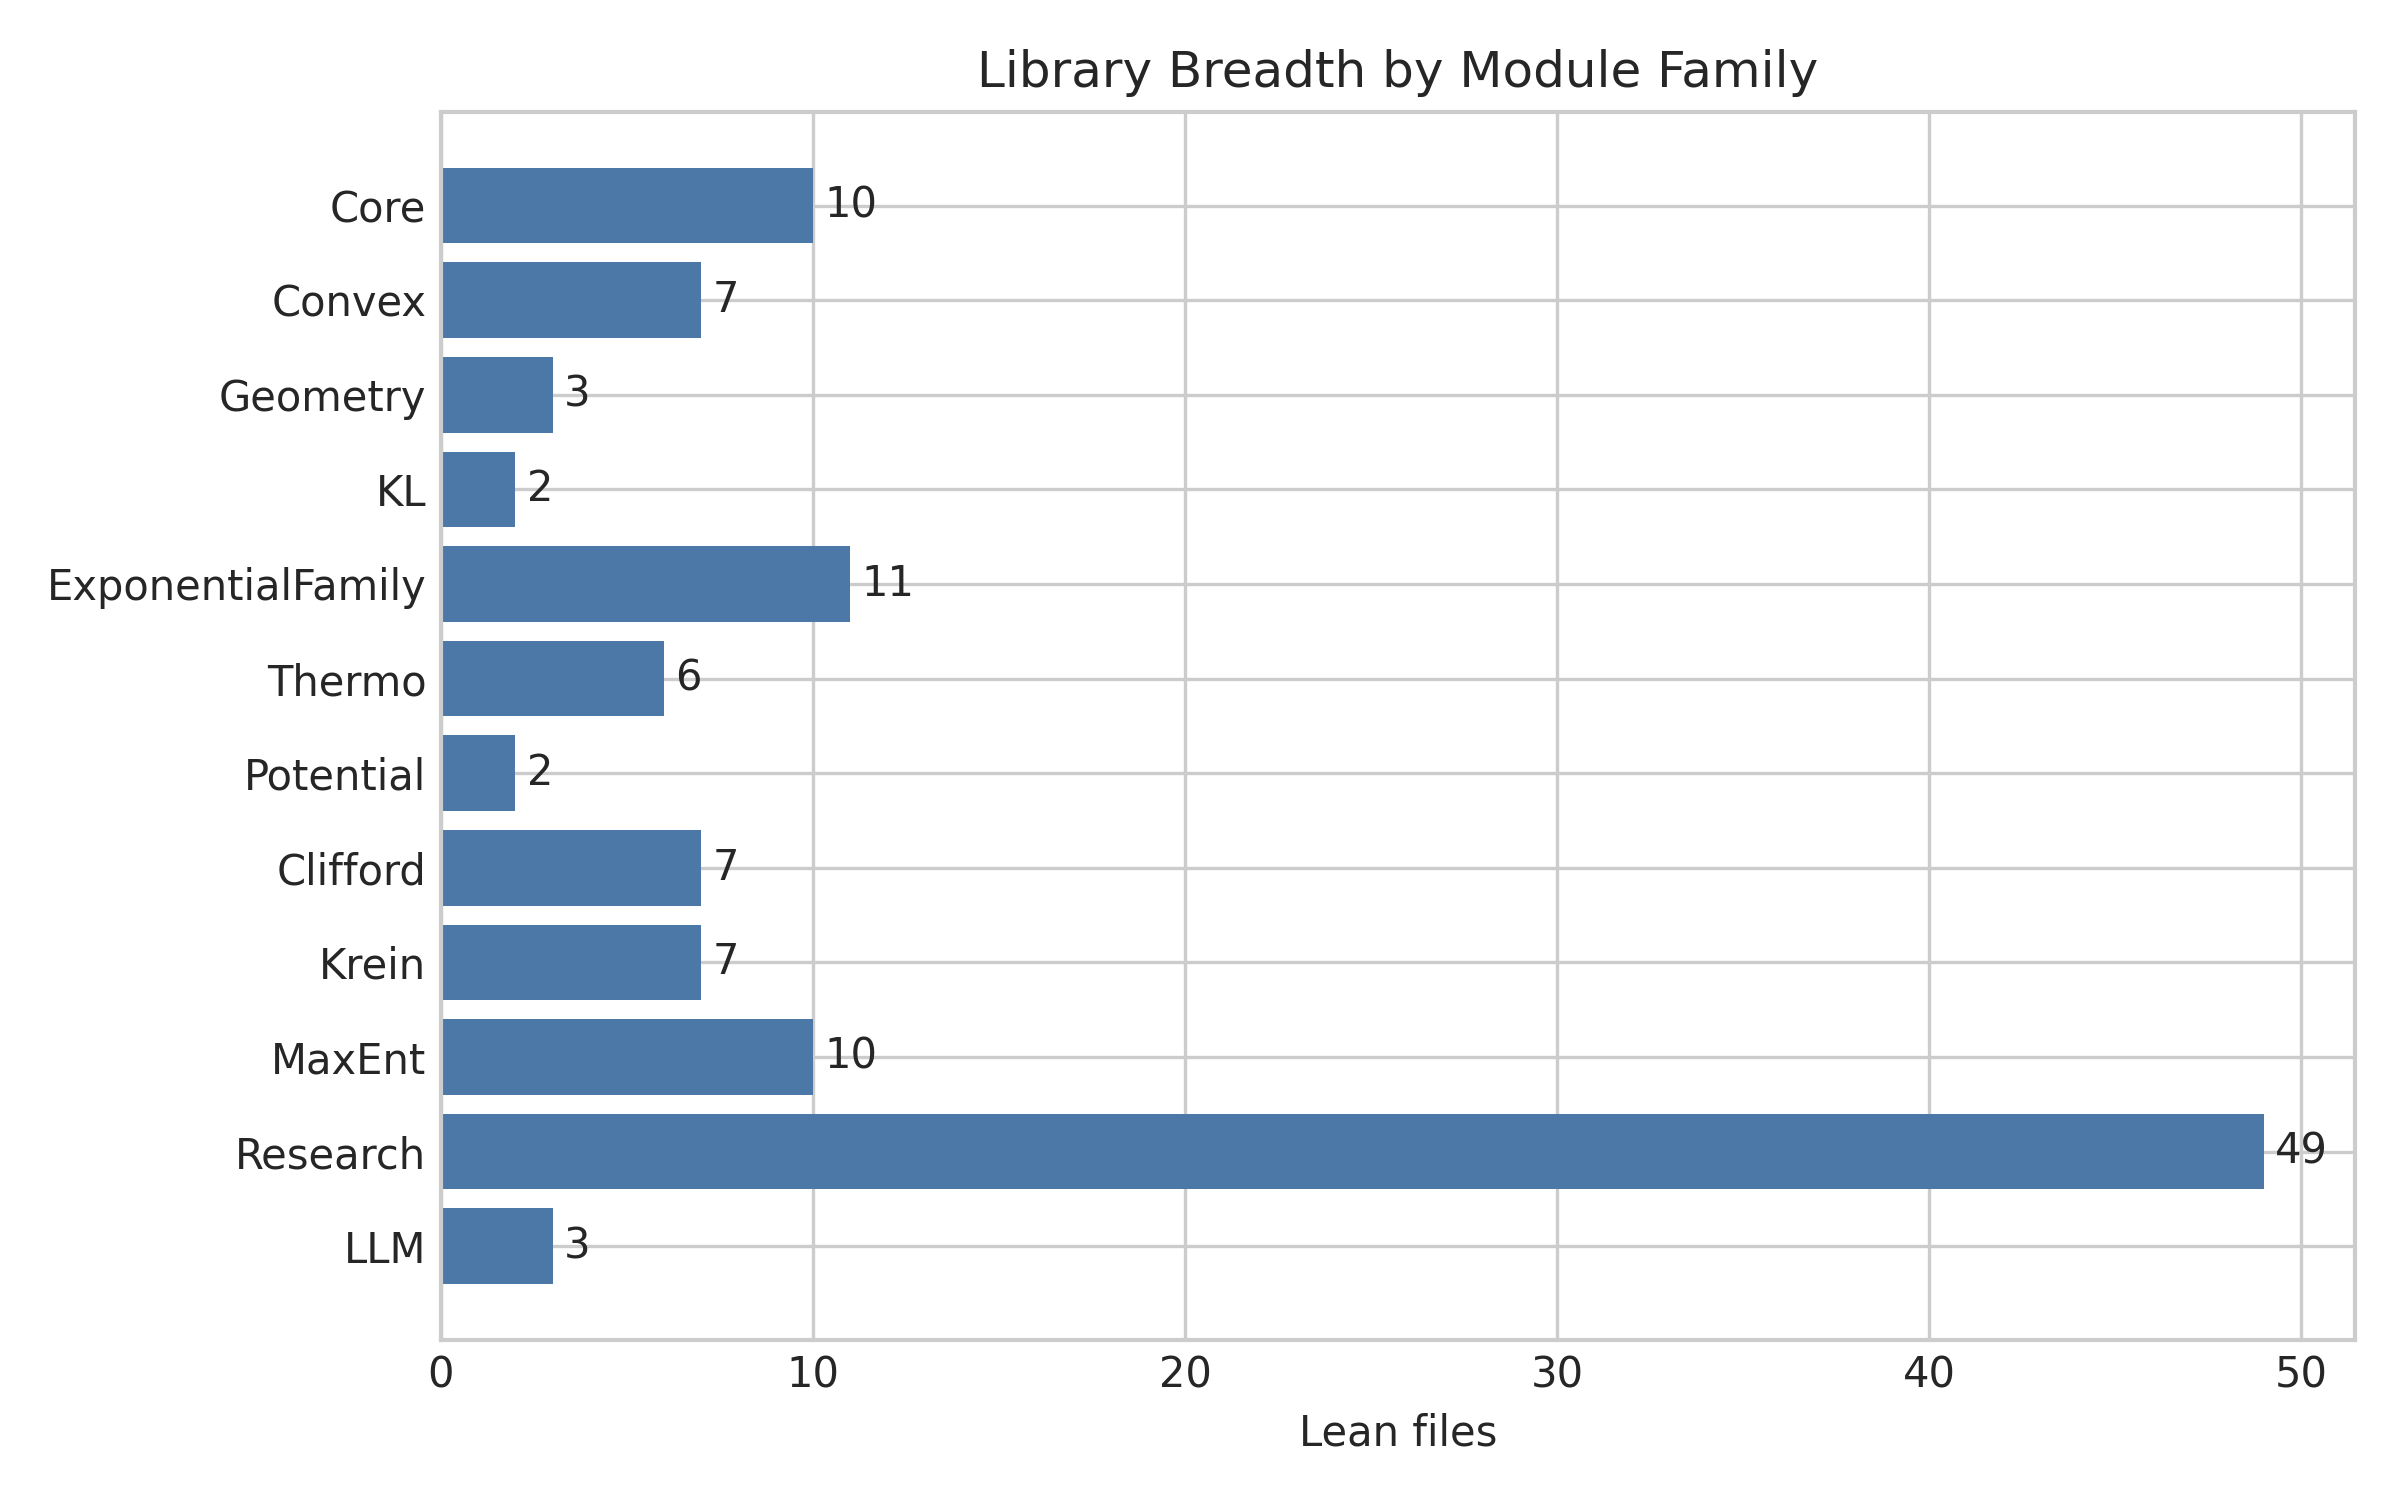
\includegraphics[height=0.62\textheight]{figures/module_coverage.png}
  \vspace{0.4em}

  \small
  Counts are generated directly from \texttt{lean/InfoGeometry/*} and expose where formal depth lives.
\end{frame}

\section{Architecture}

\begin{frame}{Canonical Layered Architecture}
  \begin{itemize}
    \item \textbf{Foundations}: \texttt{Core}, \texttt{KL}, \texttt{Convex}, \texttt{Potential}.
    \item \textbf{Statistical Geometry}: \texttt{ExponentialFamily}, \texttt{Geometry}, \texttt{Thermo}.
    \item \textbf{Operator/Algebraic Layers}: \texttt{Clifford}, \texttt{Krein}, \texttt{Prequantum}, \texttt{Quantum}.
    \item \textbf{Research incubator}: \texttt{Research.*} for new constructs before canonical promotion.
    \item \textbf{LLM API layer}: \texttt{InfoGeometry.LLM} entrypoint over verified attention abstractions.
  \end{itemize}
  \vspace{0.5em}
  \textbf{Key engineering choice}: stable canonical umbrellas + build-safe research umbrellas.
\end{frame}

\begin{frame}{Verified Cross-Domain Bridge Density}
  \centering
  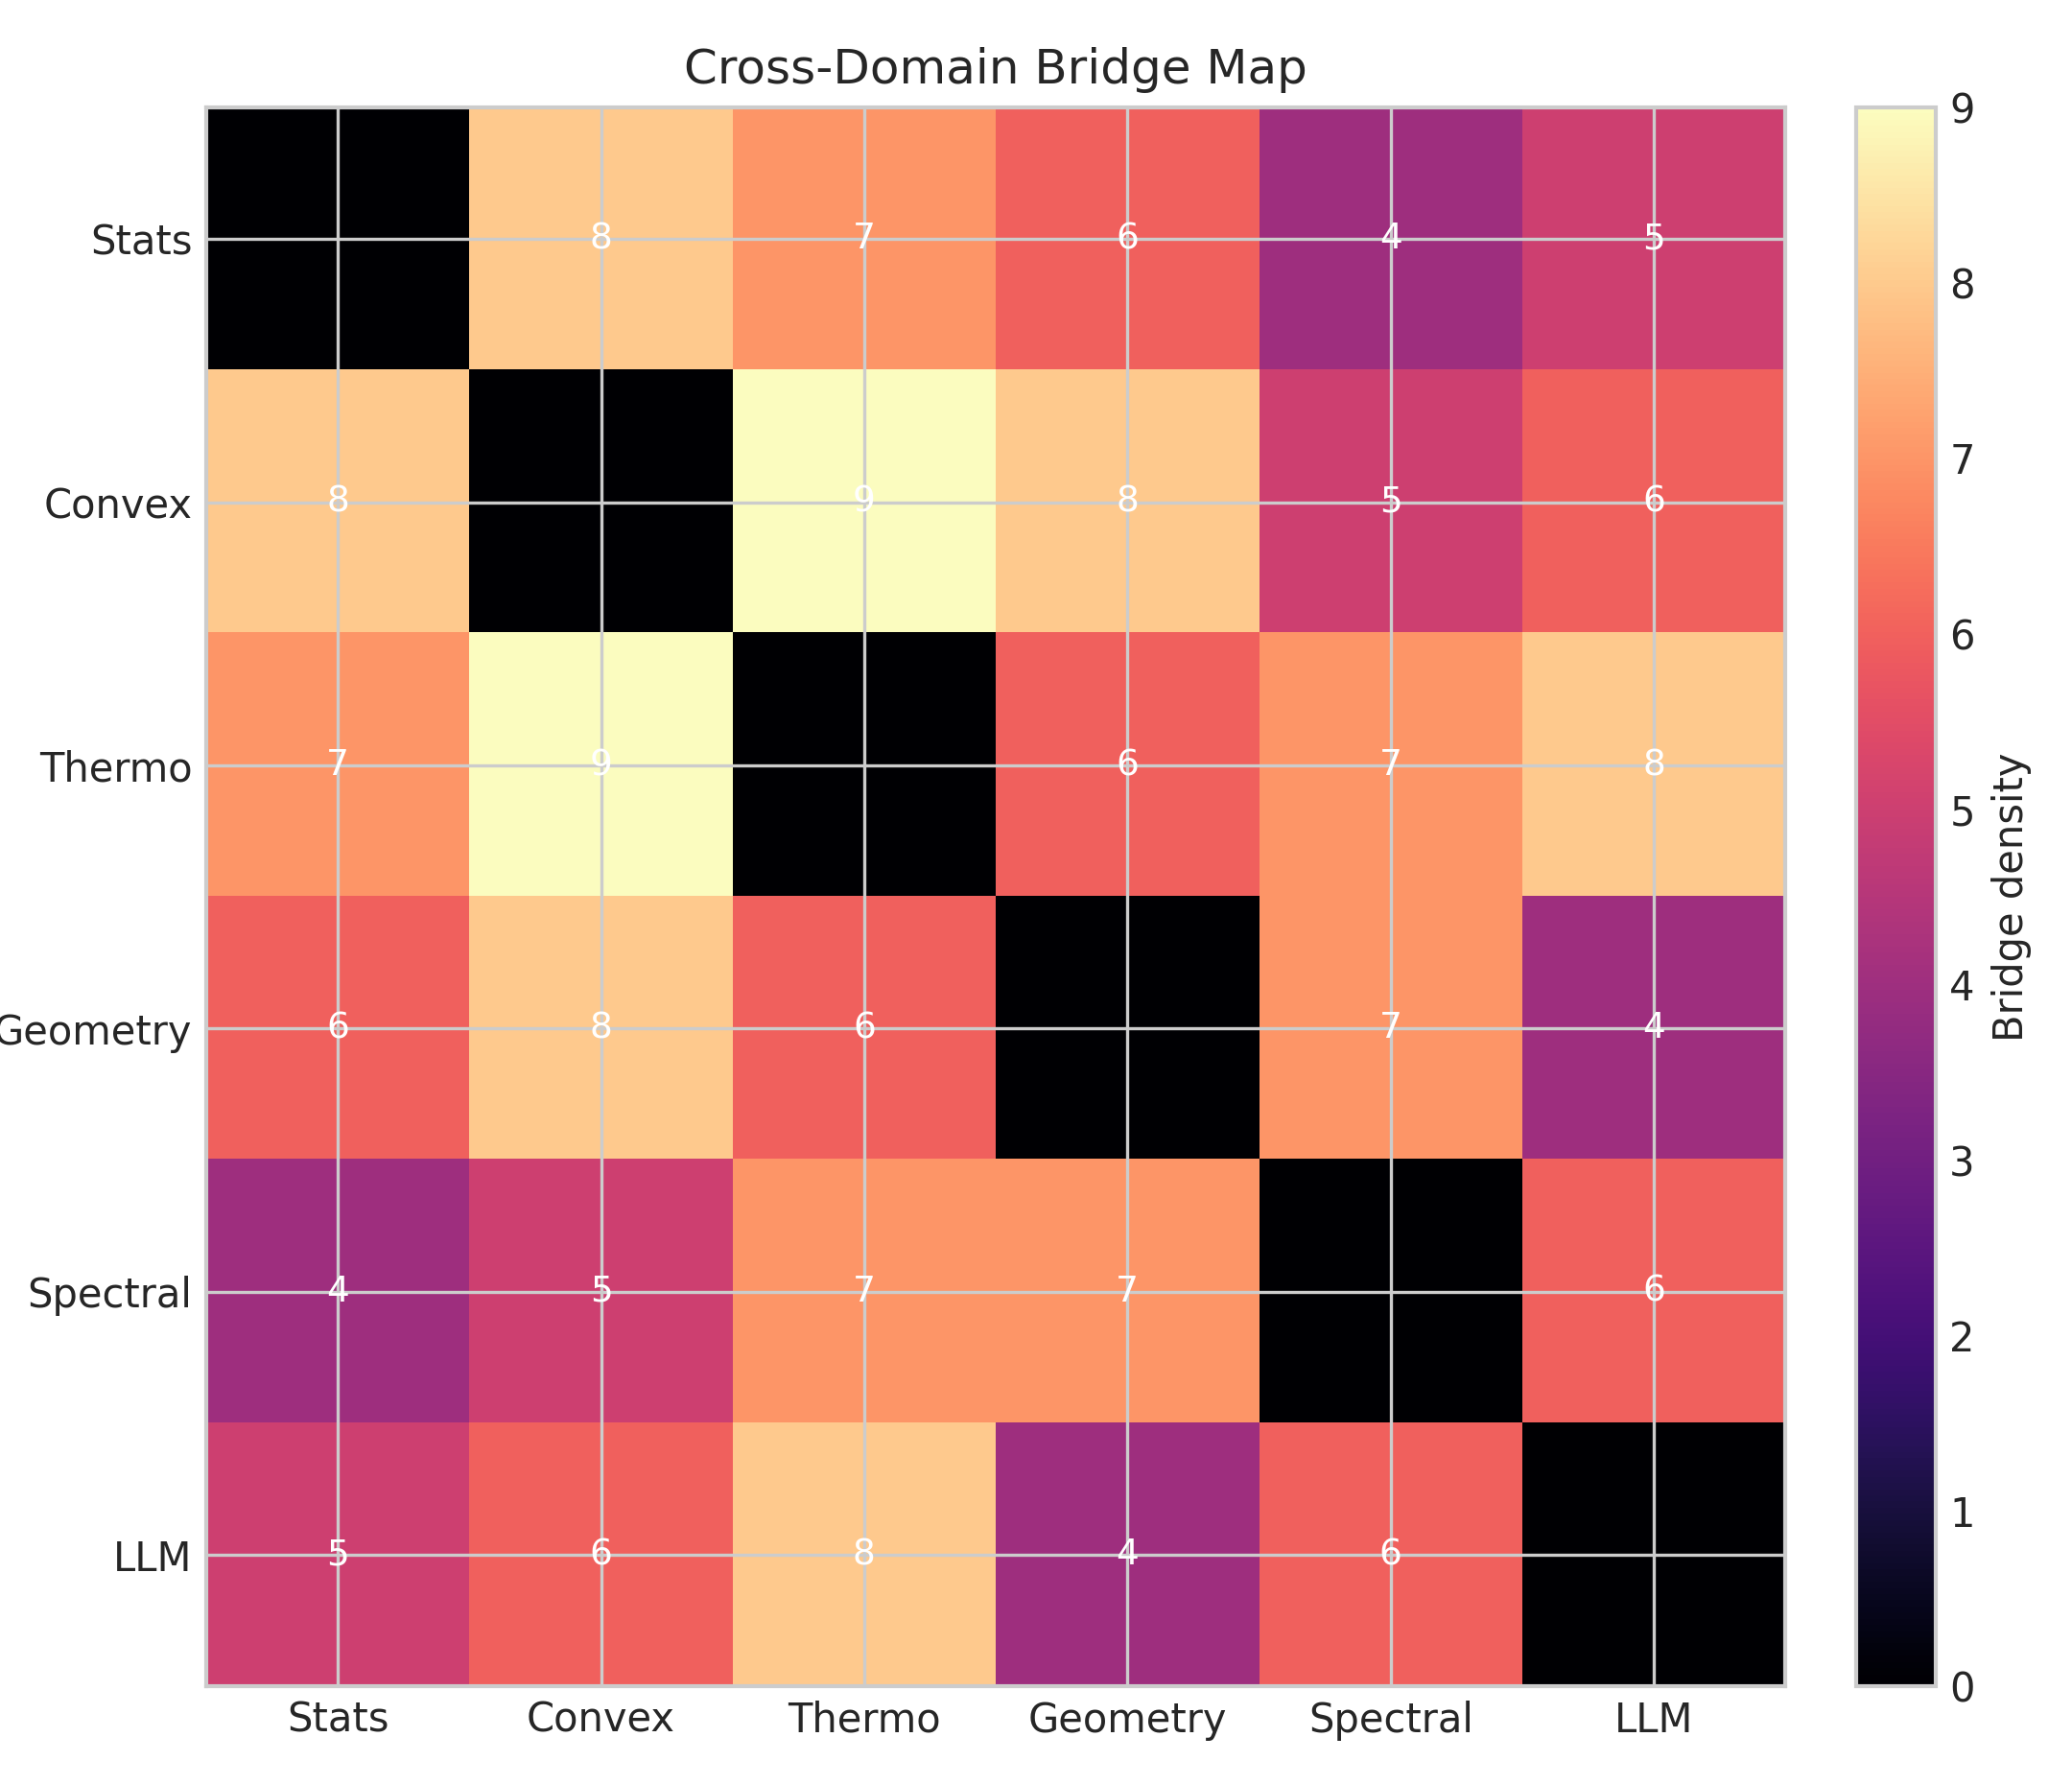
\includegraphics[height=0.62\textheight]{figures/bridge_map.png}
  \vspace{0.4em}

  \small
  The central pattern is reusable: KL/convex duality + Gibbs normalization + operator traces.
\end{frame}

\section{Core Mathematical Stack}

\begin{frame}{KL, Bregman, and Convex Potentials}
  \begin{columns}[T]
    \begin{column}{0.53\textwidth}
      \textbf{Core statement pattern}
      \[
      D_{KL}(P\Vert Q)
      =
      \nabla\text{-generated Bregman gap}
      \]
      \vspace{-0.5em}
      \begin{itemize}
        \item Finite KL formalization and nonnegativity.
        \item Bregman generators from log-partition potentials.
        \item Exponential-family bridge theorems (\texttt{KLBregman}).
      \end{itemize}
    \end{column}
    \begin{column}{0.45\textwidth}
      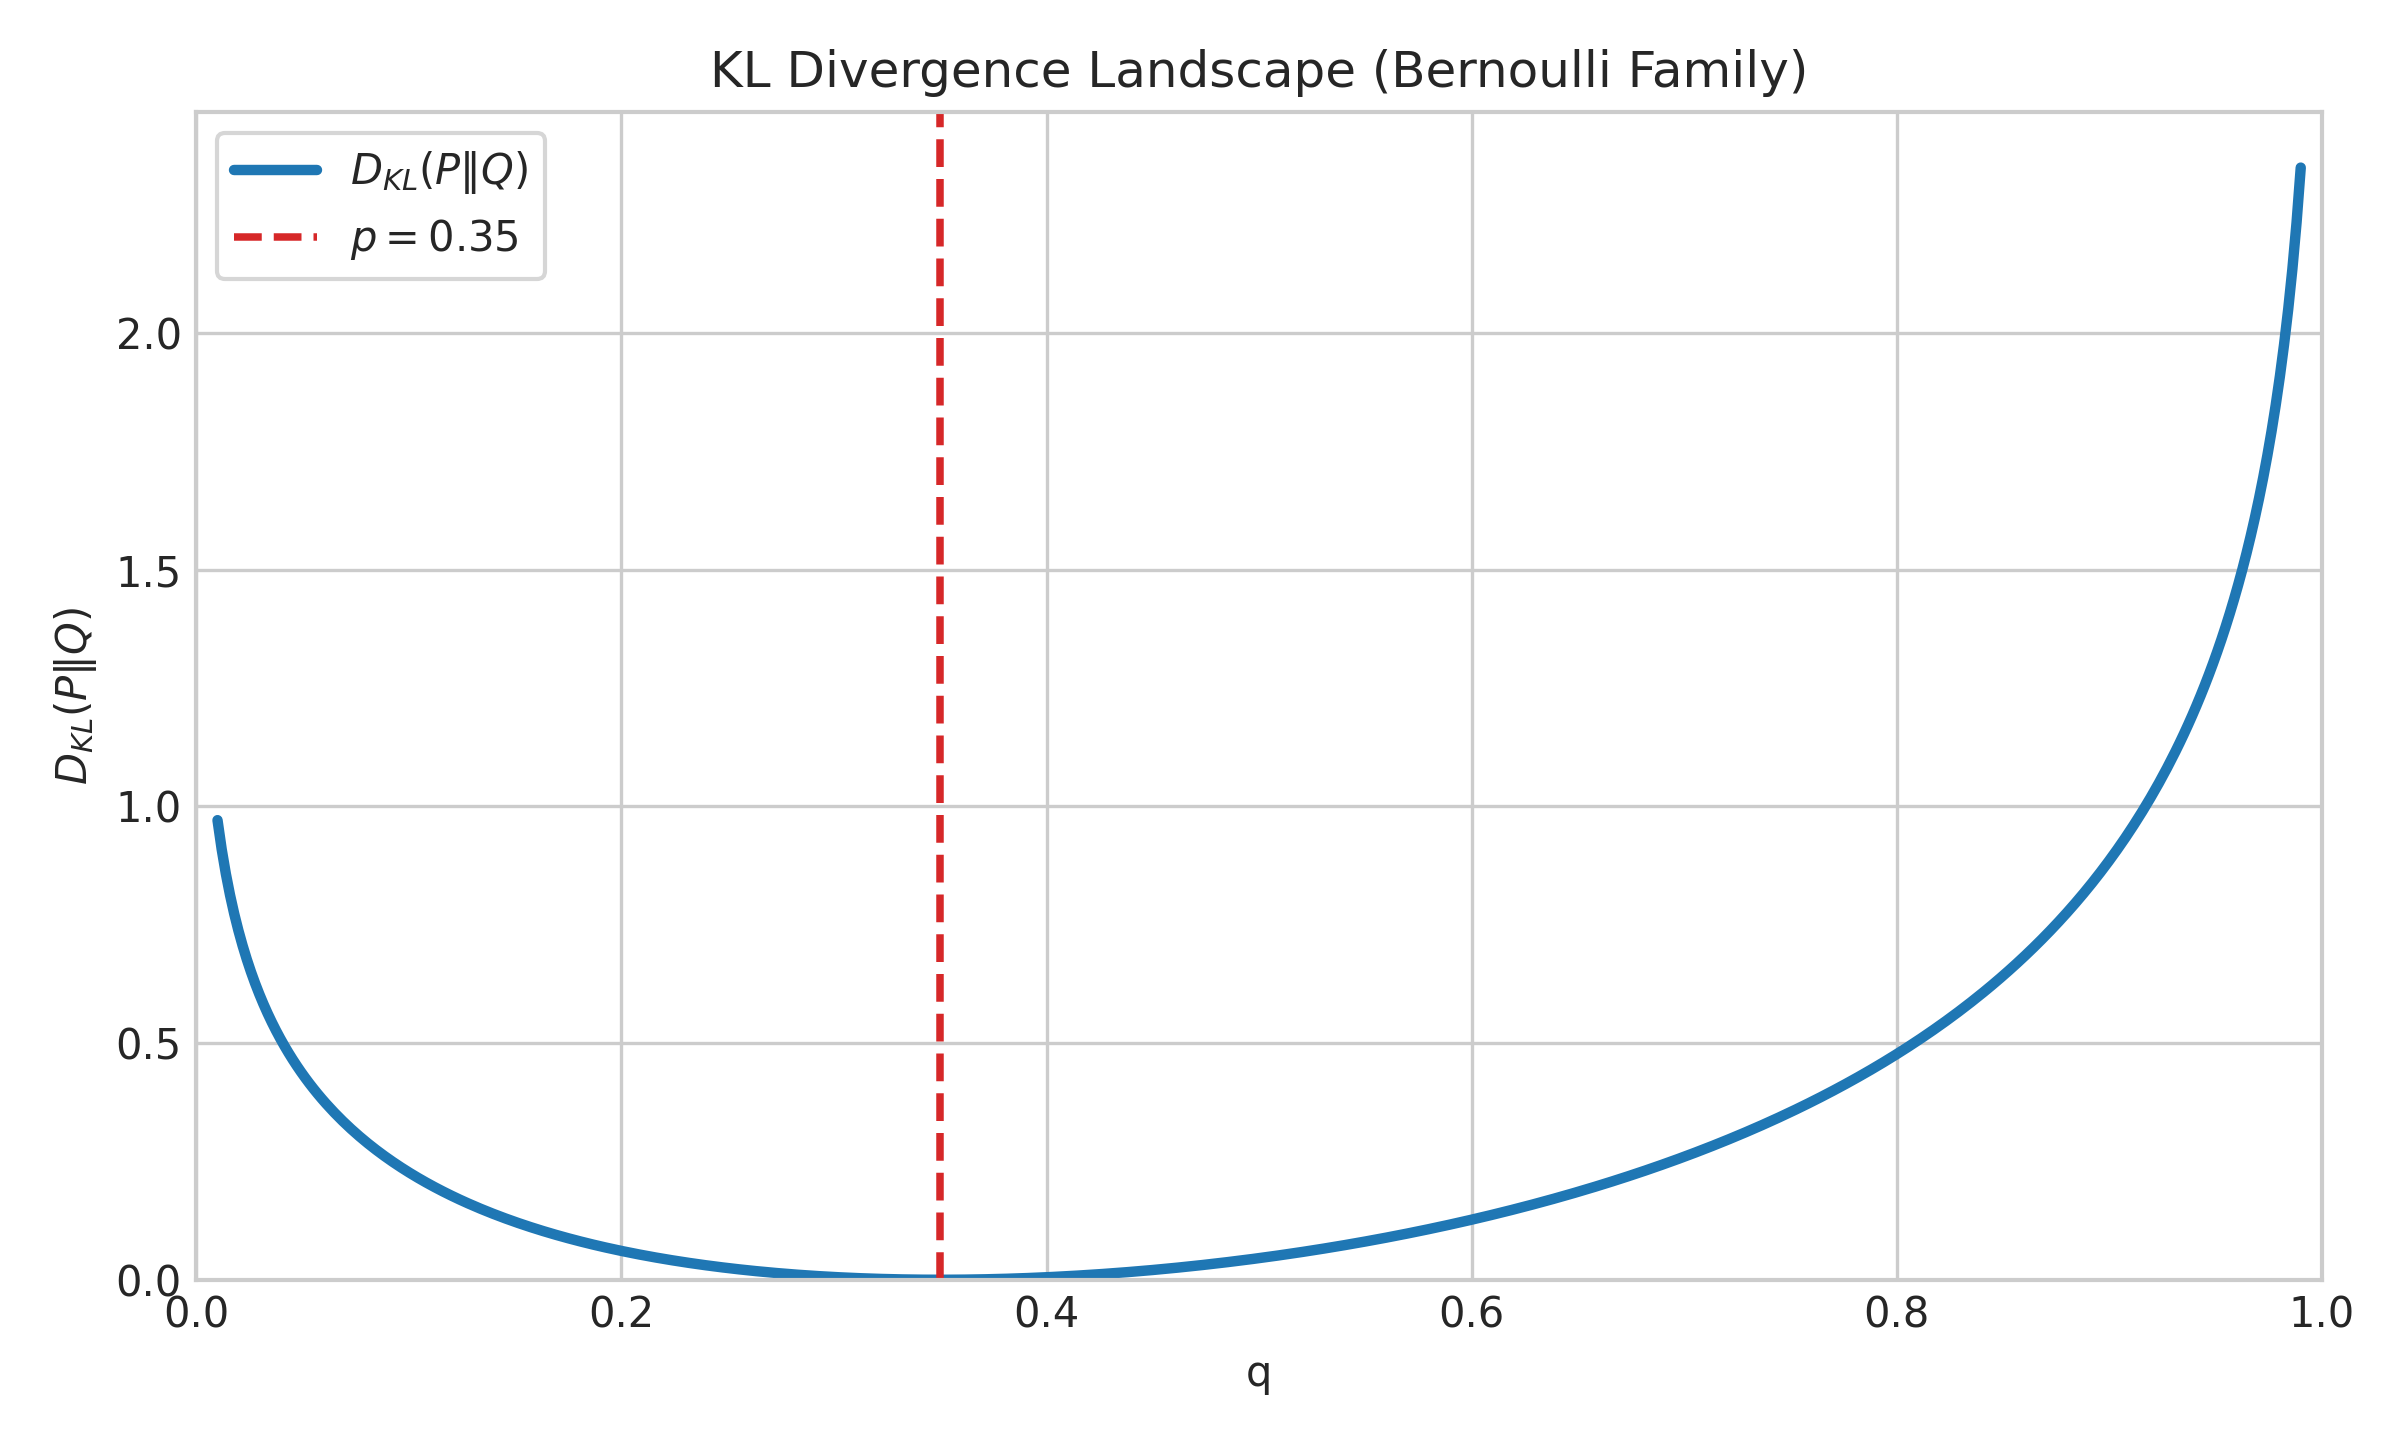
\includegraphics[width=\textwidth]{figures/kl_divergence.png}
    \end{column}
  \end{columns}
\end{frame}

\begin{frame}{Fisher Metric as Local Curvature}
  \begin{columns}[T]
    \begin{column}{0.50\textwidth}
      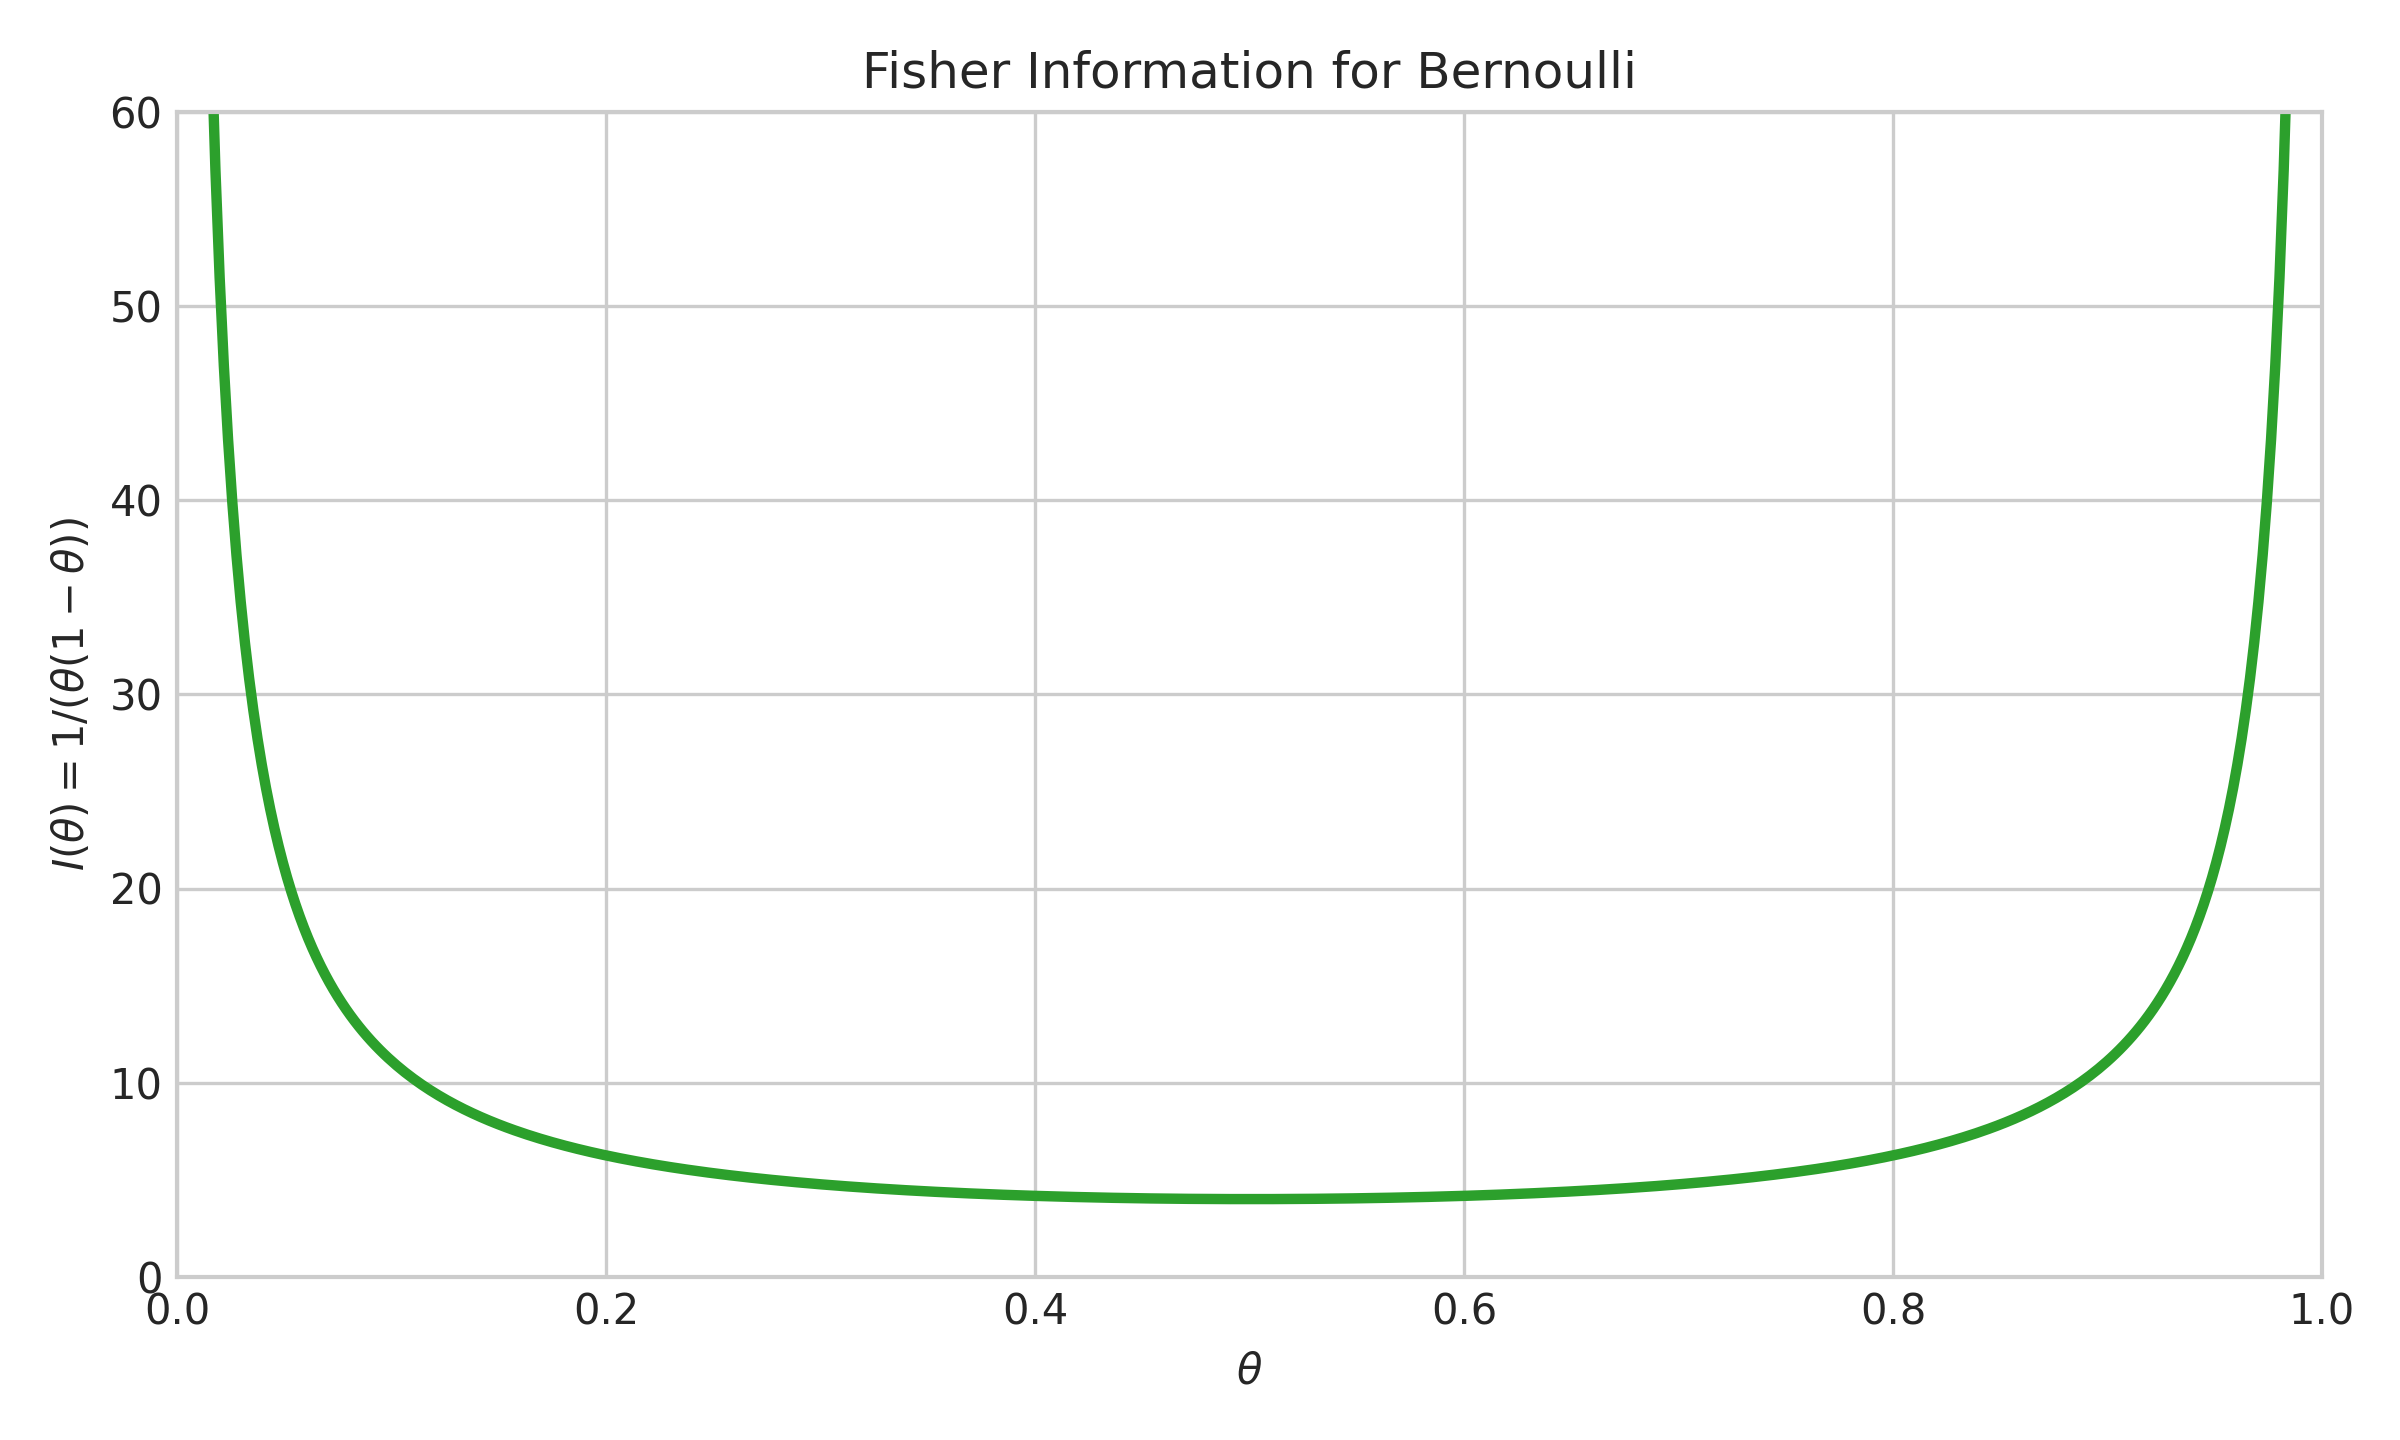
\includegraphics[width=\textwidth]{figures/fisher_info.png}
    \end{column}
    \begin{column}{0.48\textwidth}
      \[
      g_{ij}(\theta)=
      \mathbb{E}_{\theta}
      \left[
      \partial_i \log p_\theta \;
      \partial_j \log p_\theta
      \right]
      \]
      \begin{itemize}
        \item Used as metric operator in Hessian geometry packages.
        \item Drives spectral and flow surrogates in research modules.
      \end{itemize}
    \end{column}
  \end{columns}
\end{frame}

\begin{frame}{Thermodynamics and Entropic OT Layer}
  \begin{itemize}
    \item Gibbs weights, partition functions, and free-energy identities are first-class.
    \item OT naming layer now explicit in canonical-facing modules:
    \[
      \mathcal{L}_\varepsilon(\Pi)
      = \langle C,\Pi\rangle
      + \varepsilon \sum_{ij}\Pi_{ij}\log \Pi_{ij}
    \]
    \item Schr\"odinger bridge and Sinkhorn-Weyl gauge interpretation are formalized in research.
    \item This provides a direct bridge: \textbf{convex analysis} $\leftrightarrow$ \textbf{Bayesian updates} $\leftrightarrow$ \textbf{entropic transport}.
  \end{itemize}
\end{frame}

\begin{frame}{Entropy Geometry on Gaussian Manifold}
  \centering
  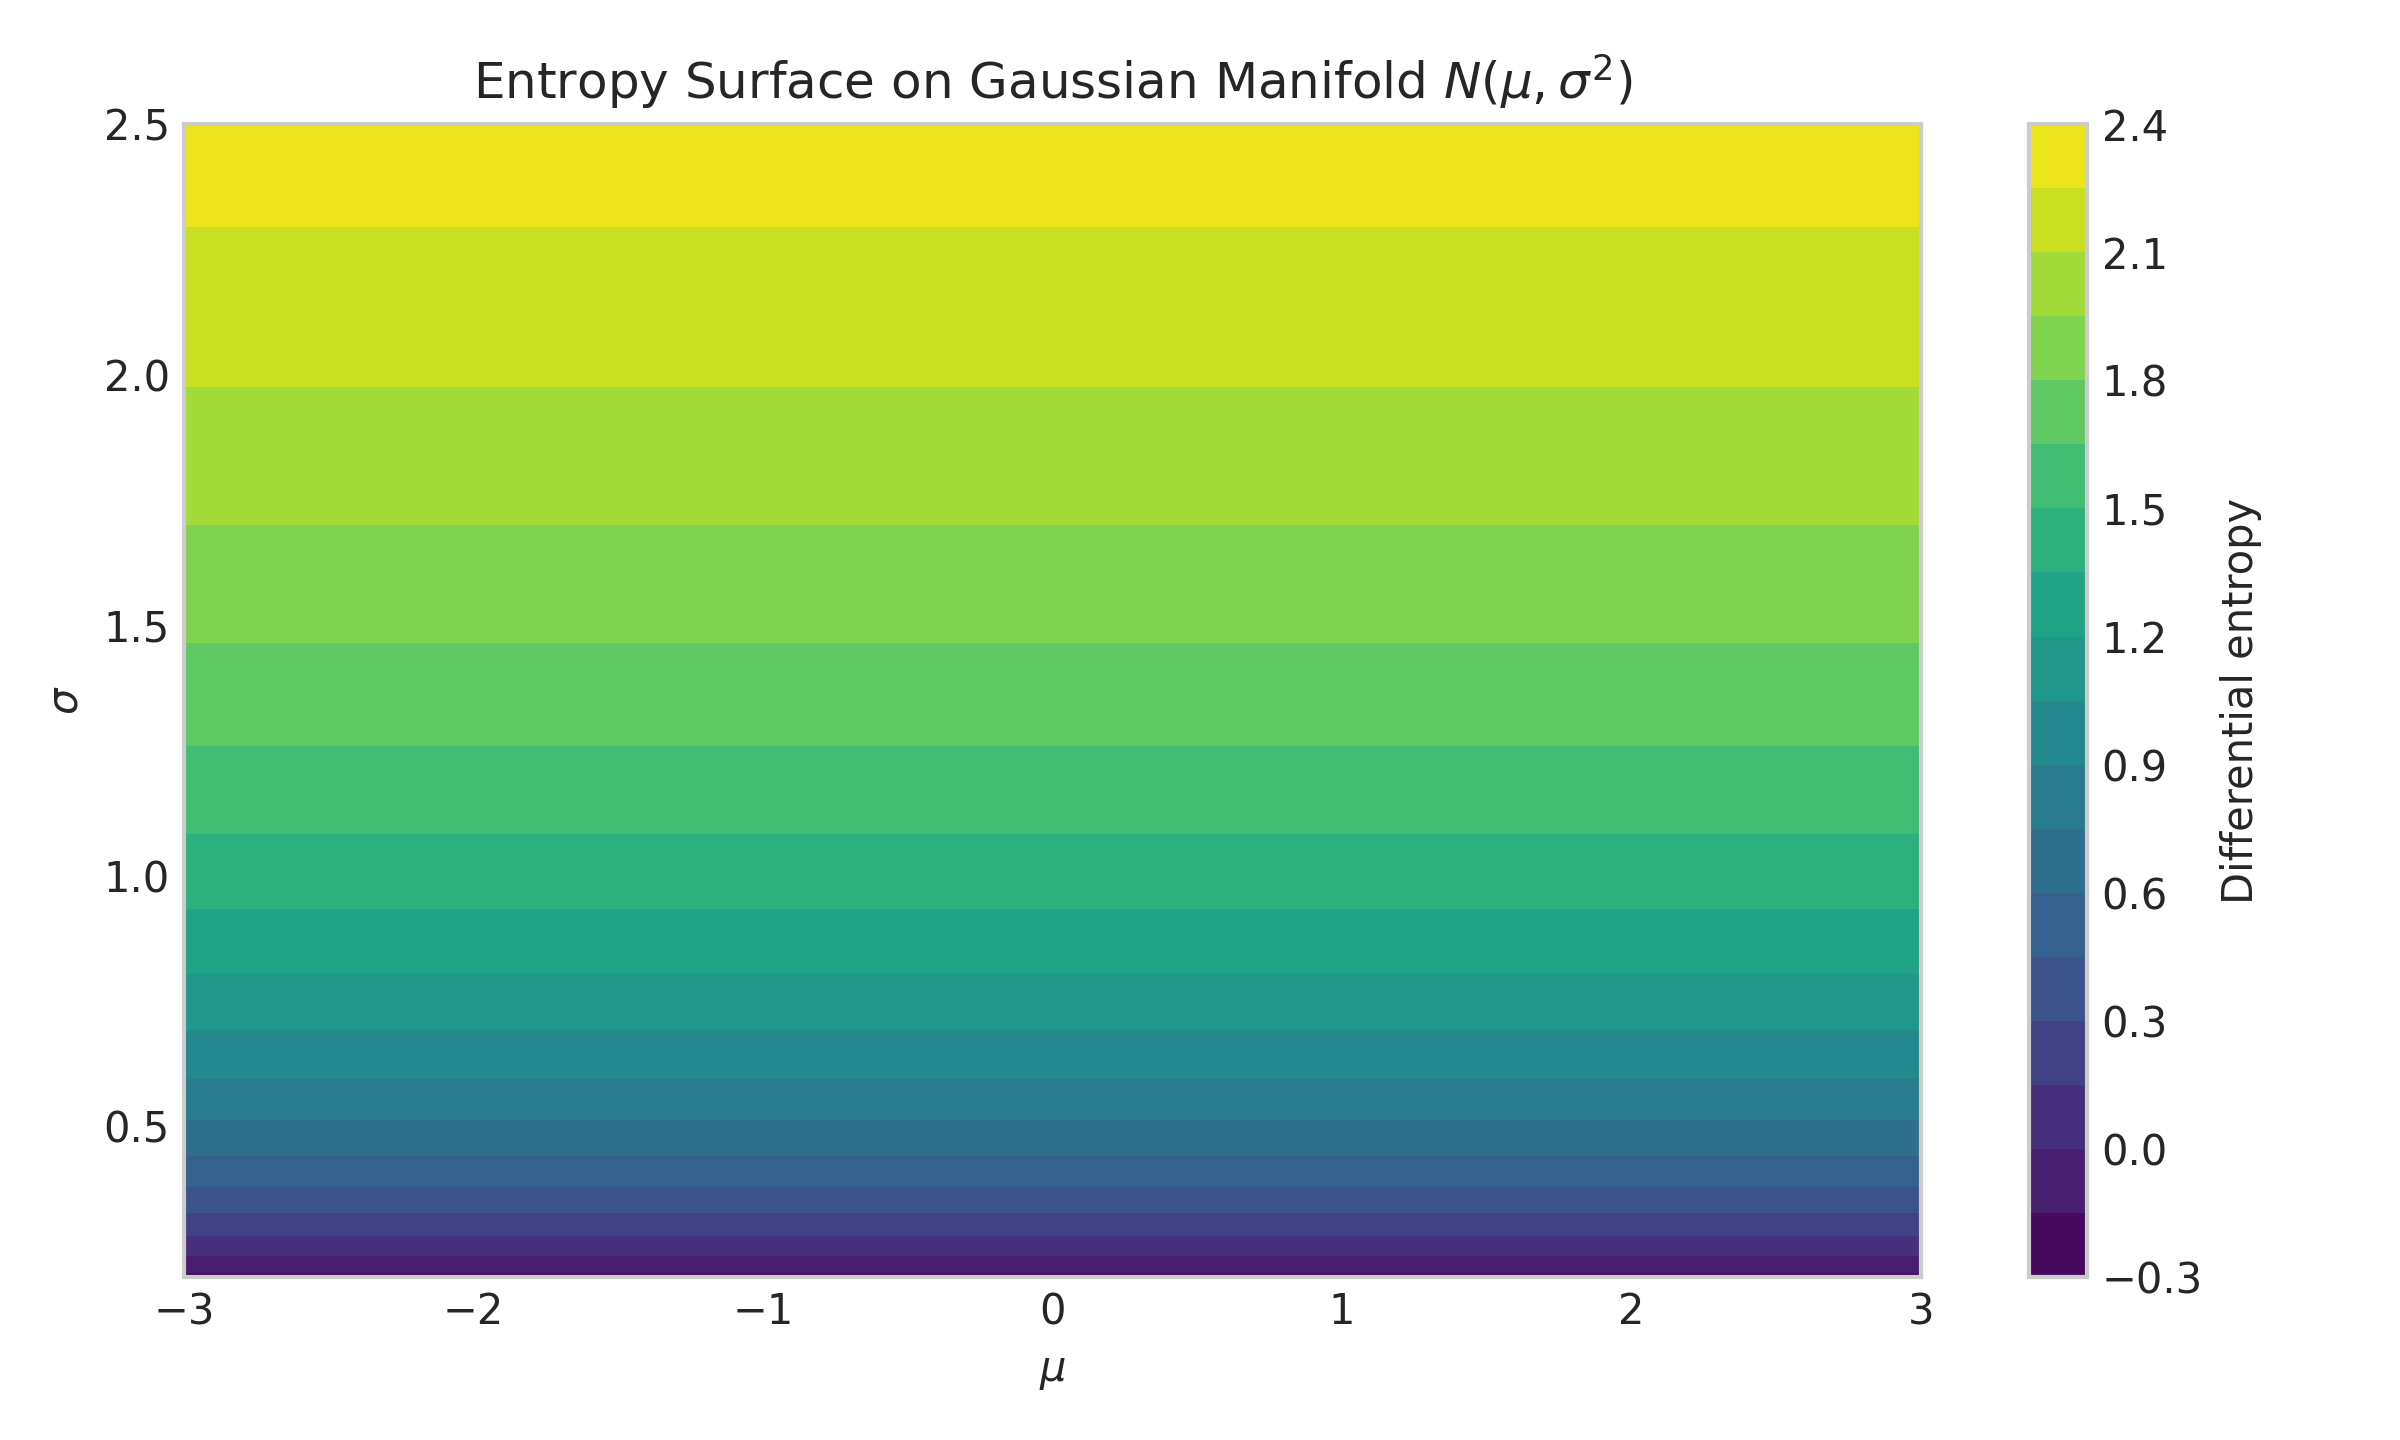
\includegraphics[width=0.74\textwidth]{figures/entropy_manifold.png}
  \vspace{0.4em}

  \small
  Geometric quantities are tied back to canonical potential and Hessian interfaces.
\end{frame}

\section{LLM Formalization Layer}

\begin{frame}{From Attention to Canonical Transformer Block}
  \centering
  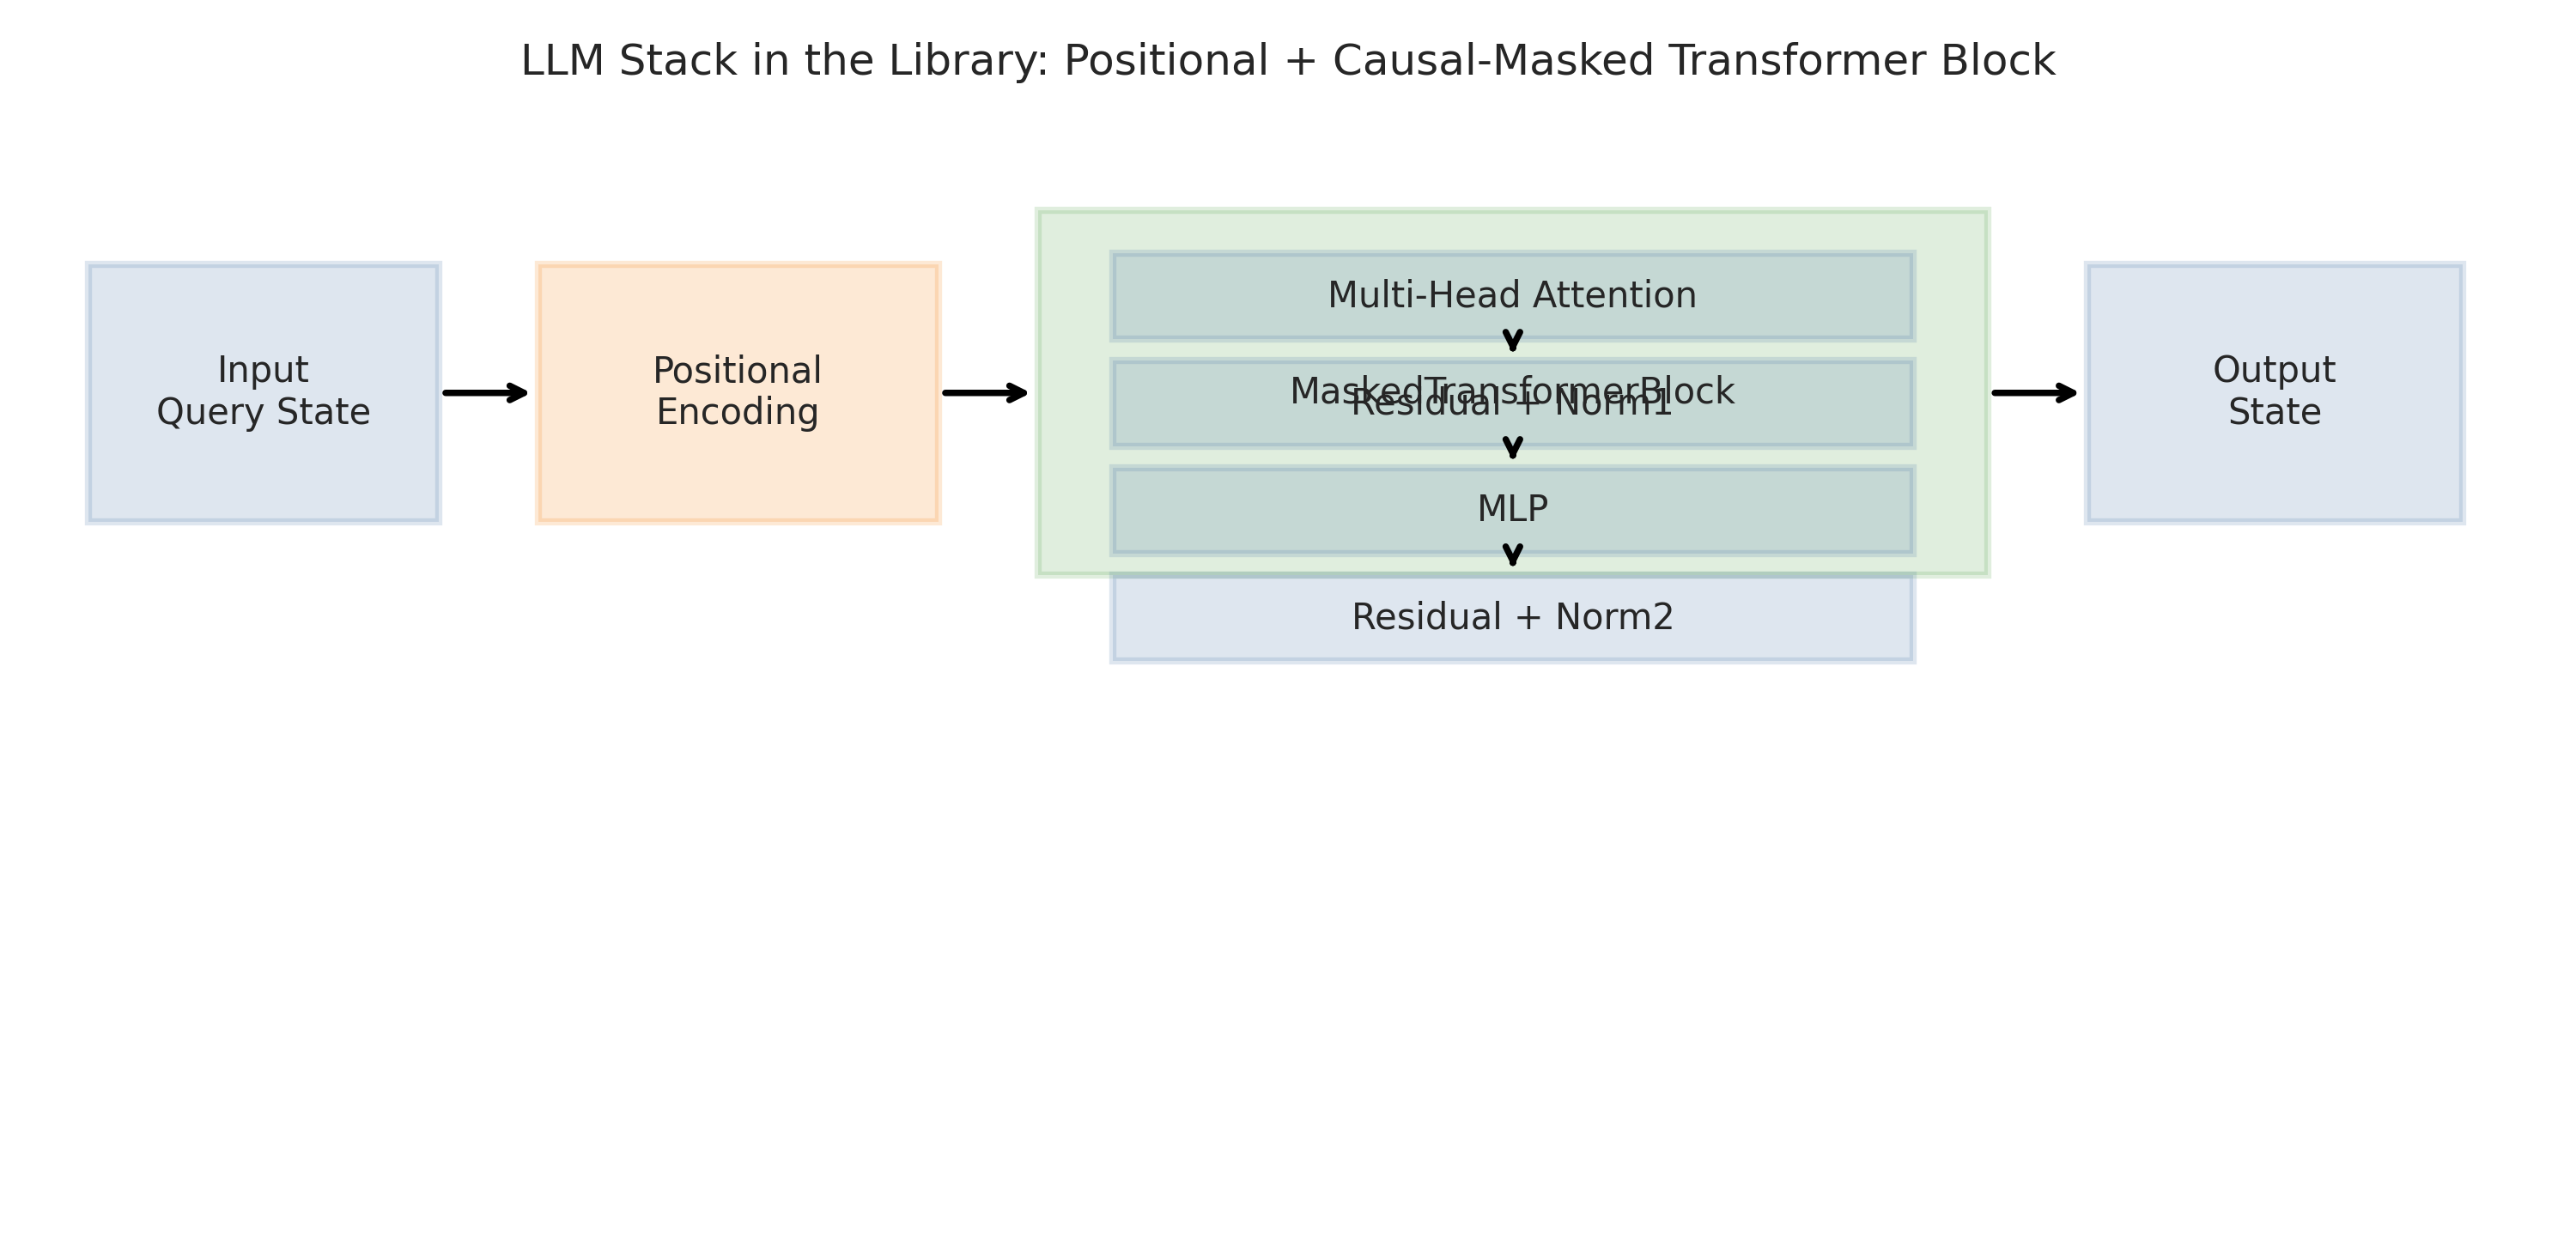
\includegraphics[height=0.62\textheight]{figures/transformer_pipeline.png}
  \vspace{0.2em}

  \small
  The new \texttt{InfoGeometry.LLM} umbrella provides reusable interfaces for
  attention, masking, residual paths, normalization, and positional composition.
\end{frame}

\begin{frame}{LLM Interfaces Added}
  \begin{itemize}
    \item \texttt{TransformerBlock}: multi-head output + residual/norm + MLP + residual/norm.
    \item \texttt{MaskedTransformerBlock}: causal-mask layer over per-head weights.
    \item \texttt{PositionalEncoding}: compositional encoding interface.
    \item Proven compatibility lemmas:
    \begin{itemize}
      \item unmasked limit recovers base run;
      \item identity encoding recovers original run;
      \item encoding composition commutes with \texttt{runWithPositionalEncoding}.
    \end{itemize}
  \end{itemize}
\end{frame}

\section{Geometric PDE and Flow Layer}

\begin{frame}{Ricci, Einstein-Kahler, and Monge-Ampere Scaffolding}
  \centering
  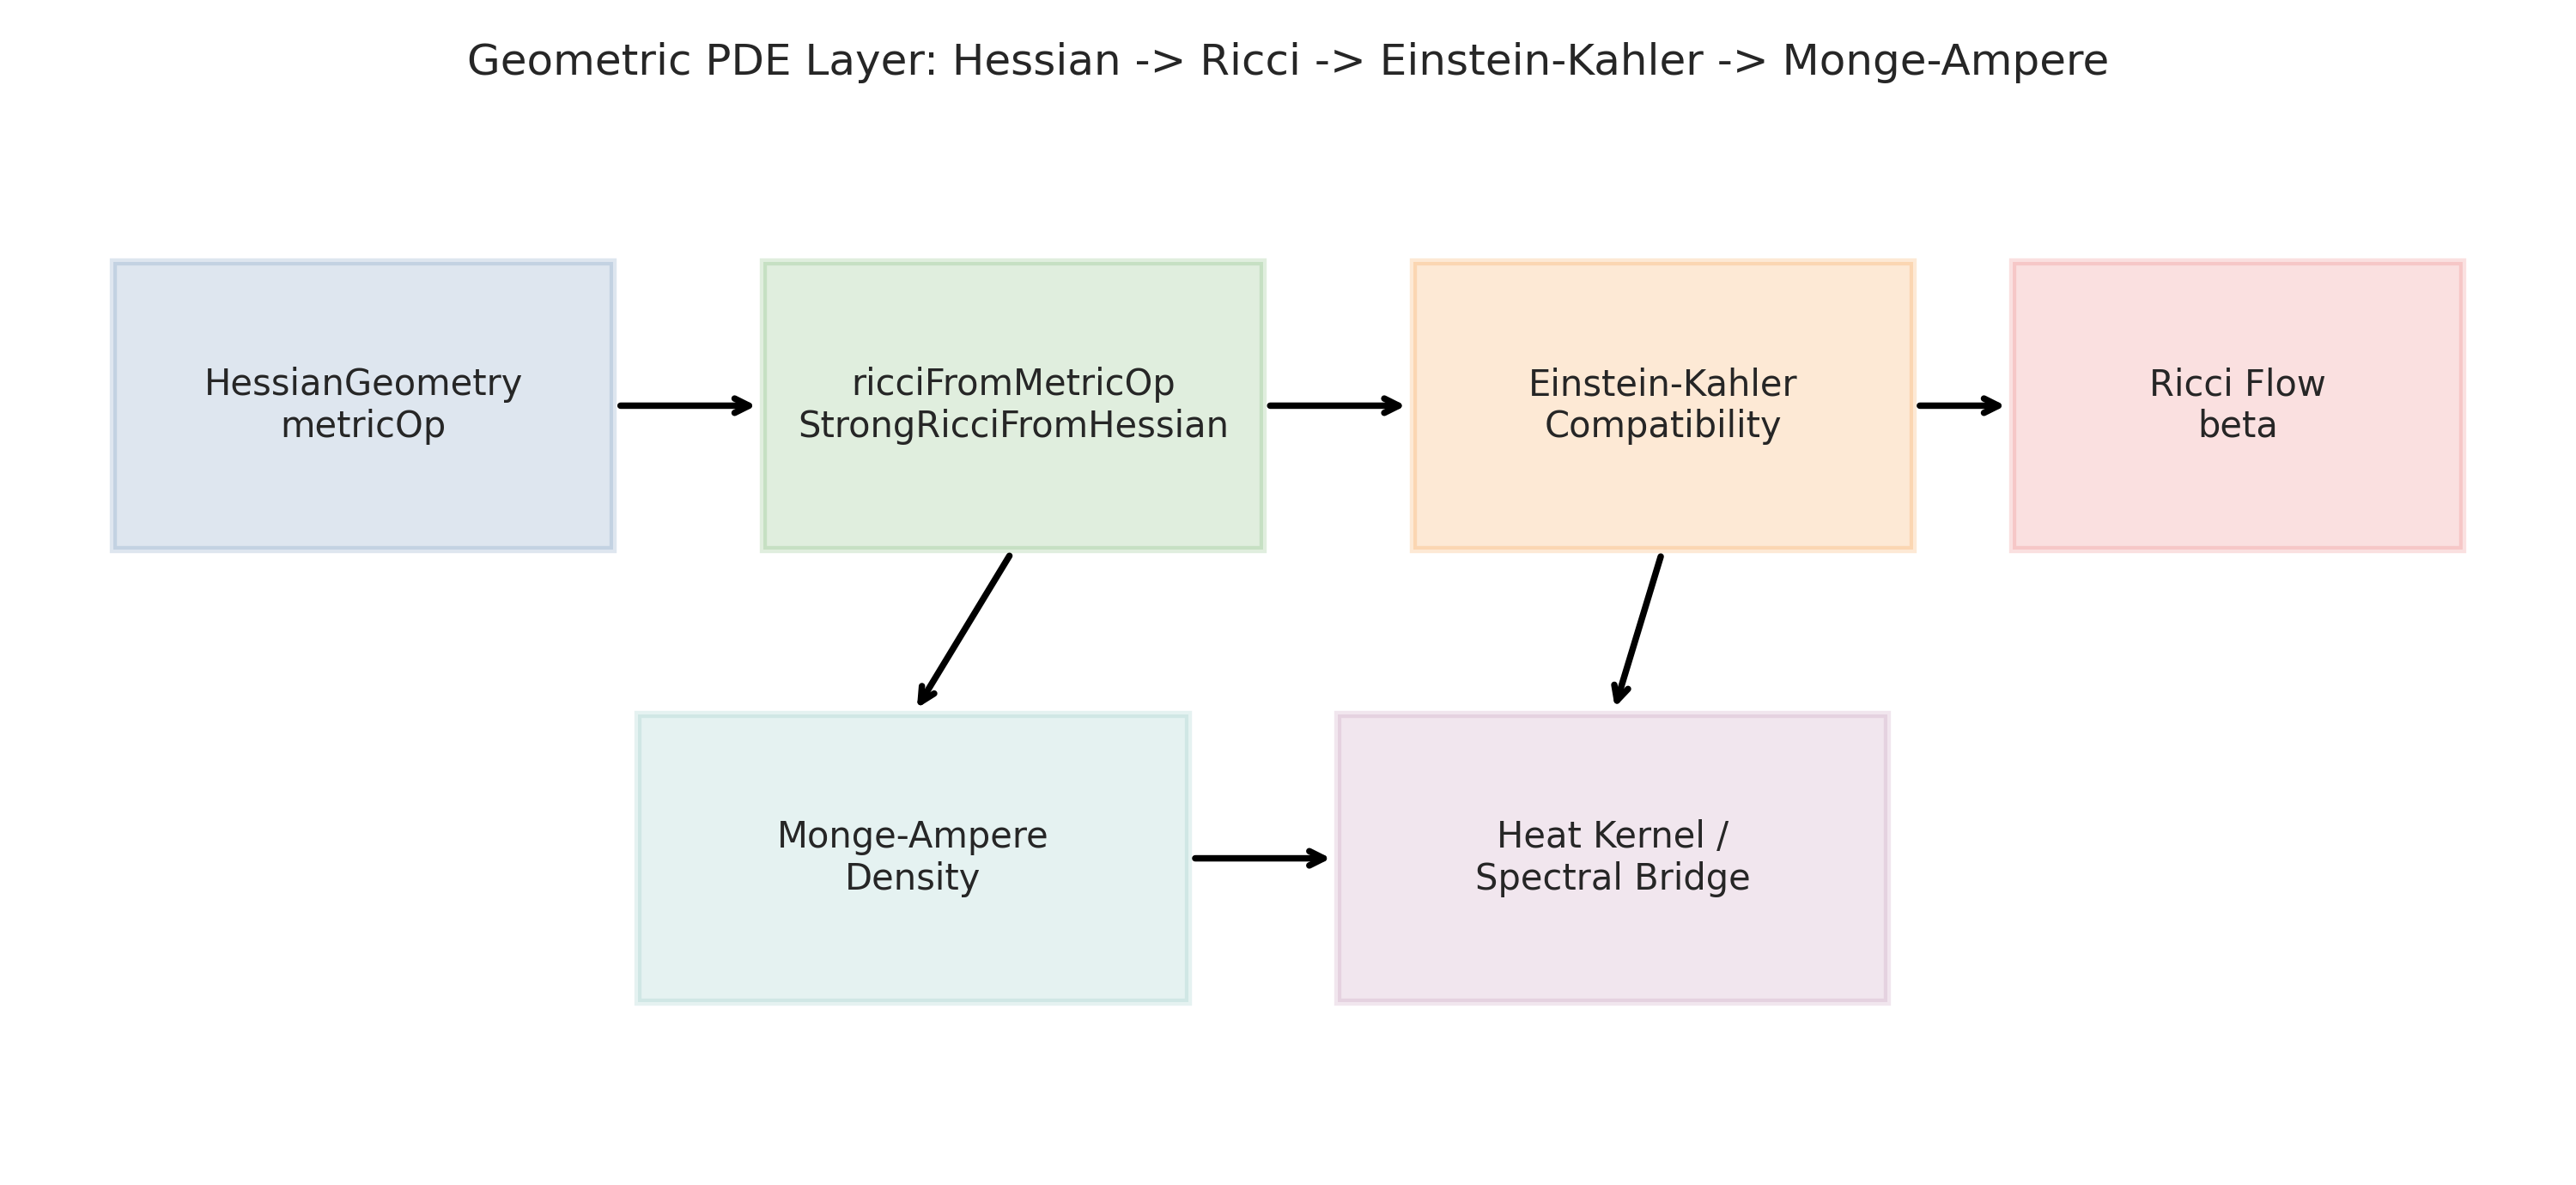
\includegraphics[height=0.62\textheight]{figures/ricci_bridge.png}
  \vspace{0.2em}

  \small
  New module \texttt{Research.RicciMongeAmpere} connects Hessian metric operators,
  scalar Ricci beta flow, and heat-kernel consistency.
\end{frame}

\begin{frame}{Flow Compatibility Statements}
  \begin{itemize}
    \item Strong Ricci object:
    \begin{itemize}
      \item metric-derived tensor from \texttt{H.metricOp},
      \item explicit symmetry and positivity hypotheses.
    \end{itemize}
    \item K\"ahler-Ricci evolution interface:
    \[
      \partial_\Lambda R(\Lambda) = \text{rhs}(\Lambda), \qquad
      \partial_\Lambda R(\Lambda) = -R(\Lambda)\;\;(\text{normalized})
    \]
    \item Compatibility lemmas tie these equations to \texttt{scalarRicciBetaFunction}.
  \end{itemize}
\end{frame}

\section{Quality Gates and Roadmap}

\begin{frame}{Verification and Integration Status}
  \begin{itemize}
    \item All presentation-related additions are build-validated with \texttt{--wfail}.
    \item Strict gate script ensures:
    \begin{itemize}
      \item canonical umbrellas elaborate cleanly,
      \item no unresolved placeholders,
      \item archive/experimental leakage checks.
    \end{itemize}
    \item Research-to-canonical promotion remains criteria-driven:
    build safety, proof completeness, semantic stability.
  \end{itemize}
\end{frame}

\begin{frame}{Next Extensions}
  \begin{itemize}
    \item Strengthen category-level abstractions for cross-domain equivalences.
    \item Expand transport/flow links into full optimal transport and geometric PDE toolkits.
    \item Add executable examples tying LLM interfaces to concrete finite models.
    \item Promote stable research modules into canonical umbrellas in staged tiers.
  \end{itemize}
  \vspace{0.8em}
  \centering
  \textbf{InfoGeometry Lean: a programmable bridge across statistics, geometry, physics, and AI.}
\end{frame}

\end{document}
